\documentclass{report}
% PACKAGES %
\usepackage[english]{} % Sets the language
\usepackage[margin=2cm]{geometry} % Sets the margin size
\usepackage{graphicx} % Enhanced package for including graphics/figures
\usepackage{float} % Allows figures and tables to be floats
\usepackage{amsmath} % Enhanced math package prepared by the American Mathematical Society
\usepackage{amssymb} % AMS symbols package
\usepackage{bm} % Allows you to use \bm{} to make any symbol bold
\usepackage{verbatim} % Allows you to include code snippets
\usepackage{setspace} % Allows you to change the spacing between lines at different points in the document
\usepackage{parskip} % Allows you alter the spacing between paragraphs
\usepackage{multicol} % Allows text division into multiple columns
\usepackage{units} % Allows fractions to be expressed diagonally instead of vertically
\usepackage{booktabs,multirow,multirow} % Gives extra table functionality
\usepackage{enumerate}
\newcommand{\tab}{\-\hspace{1.5cm}}

% Set path to figure image files
\graphicspath{ {fig/} }

% Set some custom shortcuts
\newcommand{\lap}{\nabla^2}
\newcommand{\p}{\partial}


\begin{document}

\begin{center}
\textbf{\large Nuclear Engineering 150 -- Discussion Section}\\ 
\textbf{Team Exercise Solutions \#13}
\end{center}

%%%%%%%%%%%%%%%%%%%%%%%%%%%%%%%%%% PROBLEM 1 %%%%%%%%%%%%%%%%%%%%%%%%%%%%%%%%%%
\section*{Problem 1}

A homogeneous U-235 reactor is operating at full power, 10,000 W/cm$^3$. 13\% of neutrons are absorbed in resonances, 2\% of all fission events are fast fissions, and 10\% of neutrons leak from the reactor. Assume 2.4 neutrons and 200 MeV are produced per fission, the fission cross section is 0.6 cm$^{-1}$, and the absorption cross section is 1 cm$^{-1}$.
\begin{enumerate}[a)]
\item Ignoring depletion, calculate the excess reactivity of this reactor.
\item The reactor scrams (immediately jumps to zero power). The plot below gives the negative reactivity as a function of time due to the accumulation of xenon in the reactor. Estimate at which point the reactor could no longer be returned to operation. About how long would this deadtime last?
\end{enumerate}
\begin{center}
\vspace{1cm}
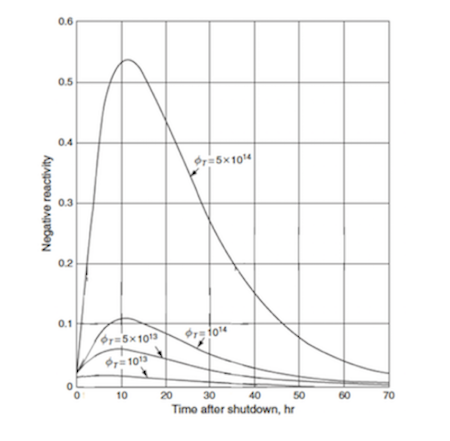
\includegraphics[width=12cm]{xenon-deadtime}
\end{center}
\vfill
$200\text{ MeV} = 3.204\times10^{-11}\text{ J}$



\section*{Problem 1 Solution}

\begin{enumerate}[a)]

\item Reactivity is defined as $\rho \equiv \frac{k - 1}{k}$. From the information provided in the problem, we can determine $k$ using the 6 factor formula. 
$$ k = \varepsilon p f \eta P_{\textit{FNL}} P_{\textit{TNL}} $$
We are told that 13\% of neutrons are absorbed in resonances, so $p = 0.87$. We are told 10\% of neutrons leak from the reactor, so $P_{\textit{NL}} = 0.9$ and we will assume $P_{\textit{NL}} = P_{\textit{FNL}} P_{\textit{TNL}}$. We are also given the fraction of fissions that are fast fissions,
$$ \frac{\Sigma_f^F}{\Sigma_f^T + \Sigma_f^F} = 0.02 ,$$
from which we can calculate the fraction of fissions that are thermal:
$$ \frac{\Sigma_f^T}{\Sigma_f^T + \Sigma_f^F} = 0.98 .$$
Noting that the definition of the fast fission factor, $\varepsilon$, is just the inverse of the thermal fission fraction, we can find a value for $\varepsilon$:
\begin{align*}
\varepsilon	&\equiv \frac{\Sigma_f^T + \Sigma_f^F}{\Sigma_f^T} \\
			&= \left(\frac{\Sigma_f^T}{\Sigma_f^T + \Sigma_f^F}\right)^{-1} \\
			&= \left(0.98\right)^{-1} \\
			&= 1.02 
\end{align*}
Finally, using the cross sections provided we determine $f$ and $\eta$. In general,
$$ \eta = \frac{\nu\Sigma_f}{\Sigma_a^{\text{fuel}}} ,$$
and for a homogeneous reactor, 
$$ f = \frac{\Sigma_a^{\text{fuel}}}{\Sigma_a} .$$
When multiplied together,
\begin{align*}
f \eta	&= \frac{\nu\Sigma_f}{\Sigma_a} \\
		&= \frac{2.4\left(0.6\text{ cm}^{-1}\right)}{1\text{ cm}^{-1}} \\
		&= 1.44
\end{align*}
Altogether,
\begin{align*}
k	&= \varepsilon p f \eta P_{\textit{FNL}} P_{\textit{TNL}} \\
	&= \left(1.02\right)\left(0.87\right)\left(1.44\right)\left(0.9\right) \\
	&= 1.15
\end{align*}
and
$$ \rho = \frac{1.15-1}{1.15} $$
$$\boxed{ \rho = 0.13 }$$

\item Having calculated a value for the reactor's excess reactivity, we can use the provided plot to find the start of the xenon-induced deadtime and its duration. The plot gives 4 curves describing the negative reactivity created by xenon in a reactor over the first few days after shutdown. Each curve corresponds to an operating flux level in the reactor. While we are not given the flux in our reactor, we can approximate it from the information given. 

We know that the reactor is producing 10,000 W/cm$^3$. This is equal to the energy produced per second, which is also equal to the product of the fission reaction rate and the energy produced per fission,
$$ P \approx E_f \Sigma_f \phi .$$
We solve this relationship for the flux (using the conversion from MeV to Joules),
\begin{align*}
\phi	&\approx \frac{P}{E_f \Sigma_f} \\
		&\approx \frac{\left(10,000\text{ W/cm}^3\right)}{\left(3.204\times10^{-11}\text{ J}\right)\left(0.6\text{ cm}^{-1}\right)} \\
		&\approx 5.2\times10^{14}\text{ cm}^{-2}\cdot\text{s}^{-1}
\end{align*}
At this flux level, we can use the top line as a reasonable approximation for our reactor's behavior. Our excess reactivity of 0.13 is shown as a dashed line on the plot, and we have added large points where our flux curve intersects our excess reactivity. When there is more negative reactivity than excess reactivity, there is no possible way to restart the reactor (even if all control rods, poisons, and absorbers are removed, the negative reactivity will surpass the excess reactivity and keep the reactor subcritical). 

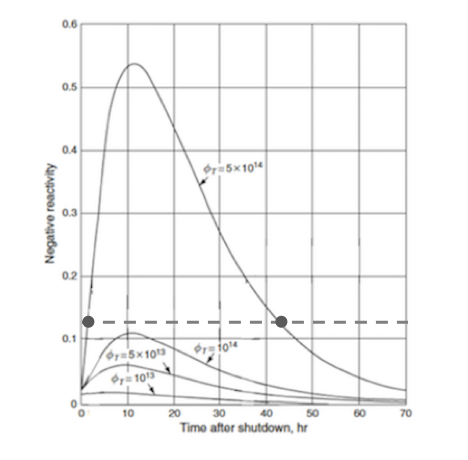
\includegraphics[width=12cm]{xenon-deadtime-marked}

The point the negative reactivity becomes greater than 0.13 and the deadtime begins is about 1 hour after shutdown. The deadtime then lasts for slightly more than 40 hours, and the reactor can be made critical again at the 42-43 hour mark.


\end{enumerate}



\newpage
%%%%%%%%%%%%%%%%%%%%%%%%%%%%%%%%%% PROBLEM 2 %%%%%%%%%%%%%%%%%%%%%%%%%%%%%%%%%%
\section*{Problem 2}

Three unknown fission products $A$, $B$ and $C$ are produced by a reactor. $B$ is stable and has a very large absorption cross section at the energies found in the reactor. The population of isotope $B$ is fed by other known fission products. Isotope $C$ decays relatively quickly into isotope $A$, which then decays again in short order. $C$ has a neglible absorption cross section, while $A$'s cross section is large. 

For each isotope, plot the behavior of the isotope's concentration after the reactor is turned on, left for a long time, then first dropped to some non-zero power, and finally shut-down.



\section*{Problem 2 Solution}

...



\end{document}

